\section{Results}
 
\subsection{The Annual Variability of Chlorophyll-a Concentration in the Korean East Sea}
 
The annual variability of chlorophyll-a concentration in the Korean East Sea from 2003~2006 is shown in Figure 1, Figure 2. Both the LAC data and the GAC data has similar tendency, showing peaks on spring(April) and fall(November). The maximum/minimum value of LAC and GAC data was each 1.61 mg/m3 / 0.28 $\rm mg/m^3$, and 1.72 $\rm mg/m^3$ / 0.32 $\rm mg/m^3$. The difference between the two data was not ignorable. This infer that the effect of spatial resolution on the data has to be considered.
  
 Figure.
 
The annual variability of 8-day-mean chlorophyll-a concentration in the Korean East Sea from 2003 to 2006 is shown in Figure 3, Figure 4. This result allowed more concrete analysis of the data. The spring peak had 1.2 ~ 1.3 $\rm mg/m^3$ of chlorophyll-a concentration and was higher than the fall peak which had the value of 0.9 ~ 1.0 $\rm mg/m^3$. Winter had a higher concentration (0.6 $\rm mg/m^3$) compared to summer (0.4 $\rm mg/m^3$). The chlorophyll-a concentration in the Korean East Sea had clear seasonal differences. Both the LAC data and the GAC data was sufficient to show the seasonal differences. However, even though the 8-day mean data was created using average of 4 years, the time of maximum concentration was different. 

Part of the LAC data (2004 46th 8-day-mean, 2005 11th 8-day mean, 2005 31th 8-day mean) had been lost due to satellite failures. The data for these dates were substituted with the average of the adjacent data. This did not have a significant effect on the tendency, so the error was ignorable.
  
  Figure.
 
The monthly-mean chlorophyll-a concentration of LAC from 2003 to 2006 is shown in Figure 5 and Figure 6. The monthly-mean chlorophyll-a concentration of GAC from 2003 to 2006 is shown in Figure 7 and Figure 8. The grey area is land showing Korea at the west and Japan at the southeast. Red means high concentration than the blue as it can be told from the color bar. Spring (March, April, May) and fall (October, November) show high concentration. The black area is part with no data due to cloud coverage or satellite failures. 
  
\begin{figure}
	\centering
	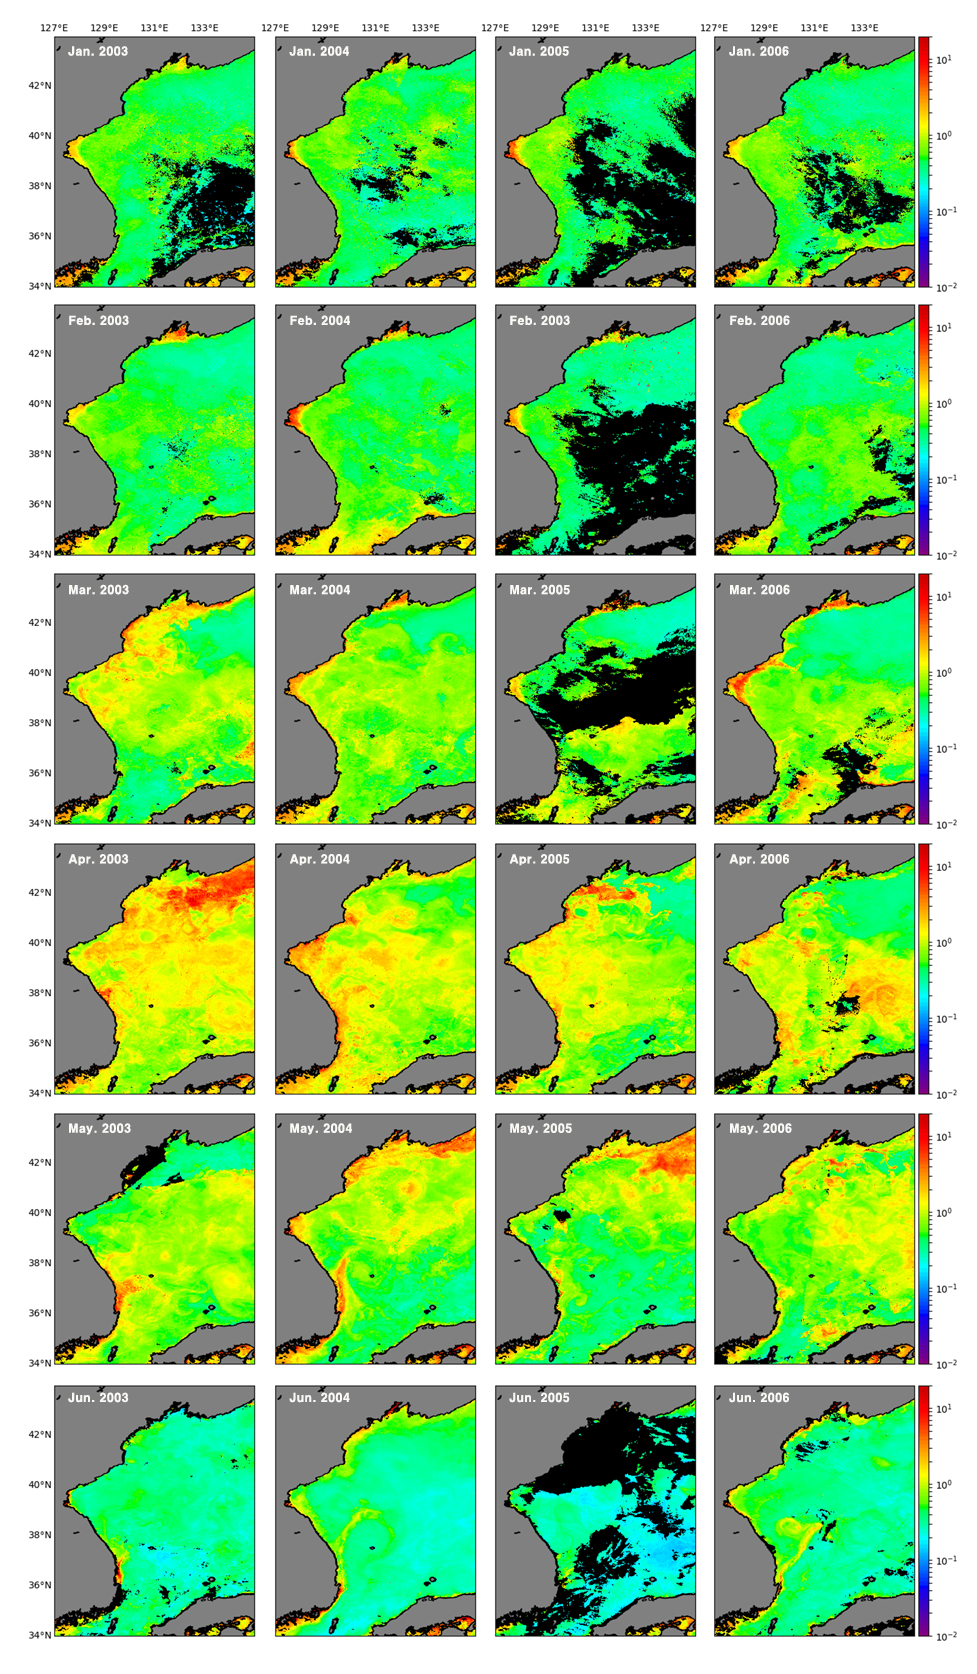
\includegraphics[width=0.8\linewidth]{../images/noname01}
	\caption{The monthly-mean chlorophyll-a distribution in the Korean East Sea, LAC. From 2003 to 2006, January to June. The unit of the color bar is $\rm mg/m^3$.}
	\label{fig:noname01}
\end{figure}
 

\begin{figure}
	\centering
	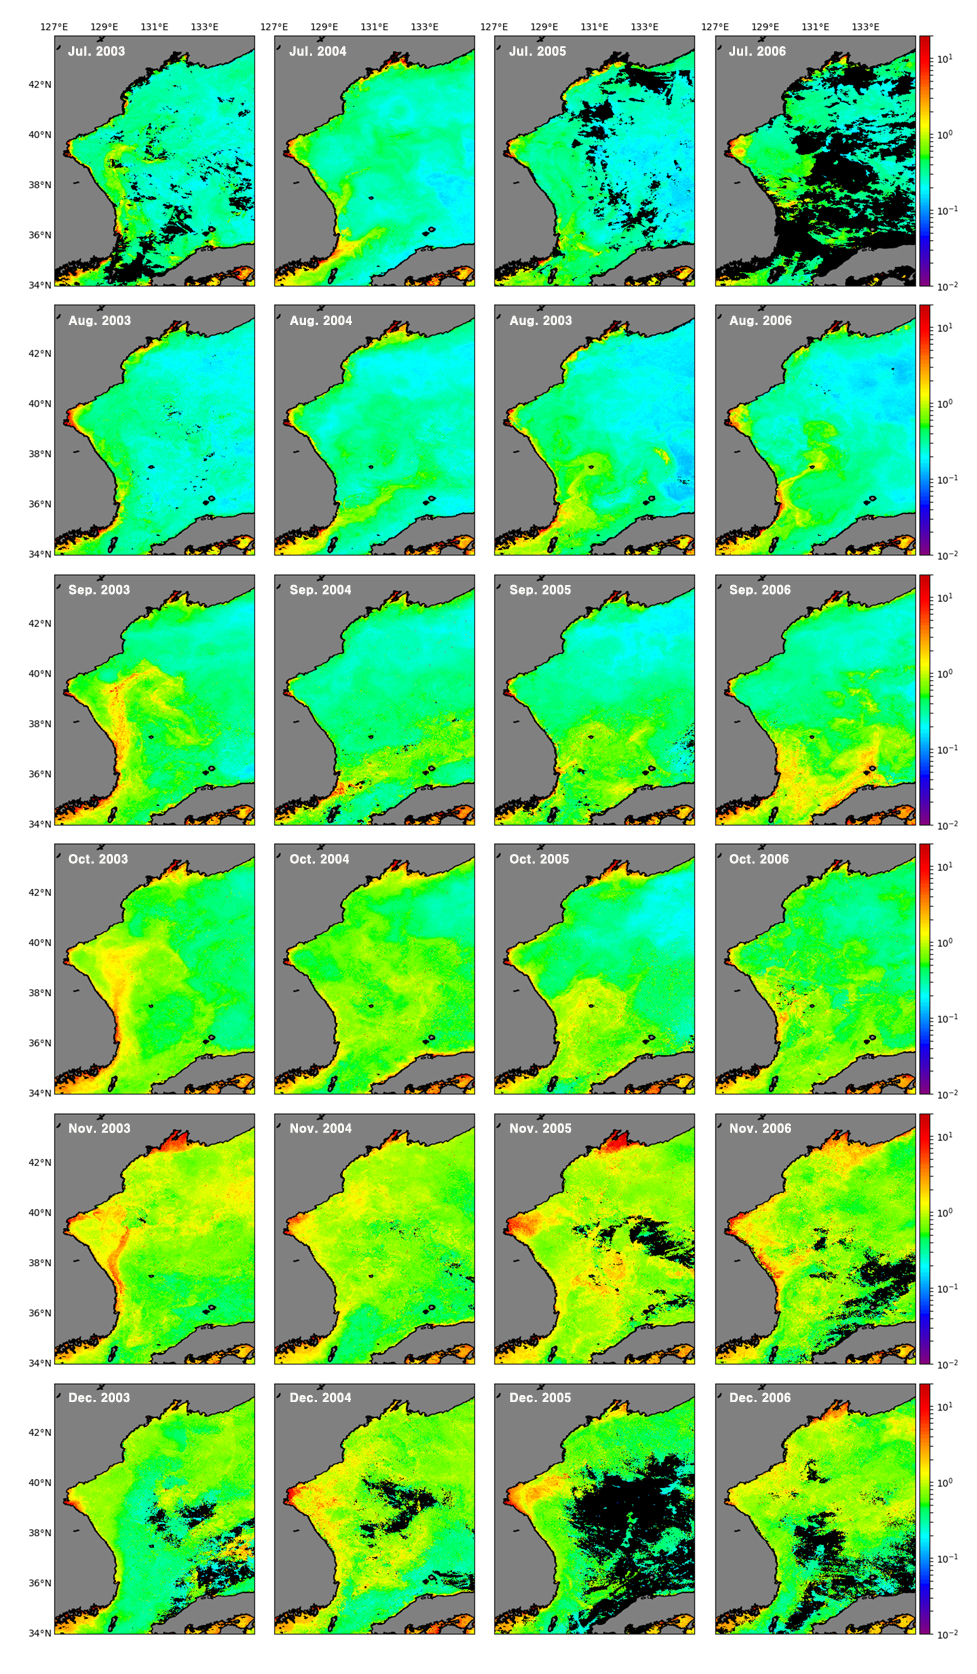
\includegraphics[width=0.8\linewidth]{../images/noname02}
	\caption{The monthly-mean chlorophyll-a distribution in the Korean East Sea, LAC. From 2003 to 2006, July to December. The unit of the color bar is $\rm mg/m^3$.}
	\label{fig:noname02}
\end{figure}

\begin{figure}
	\centering
	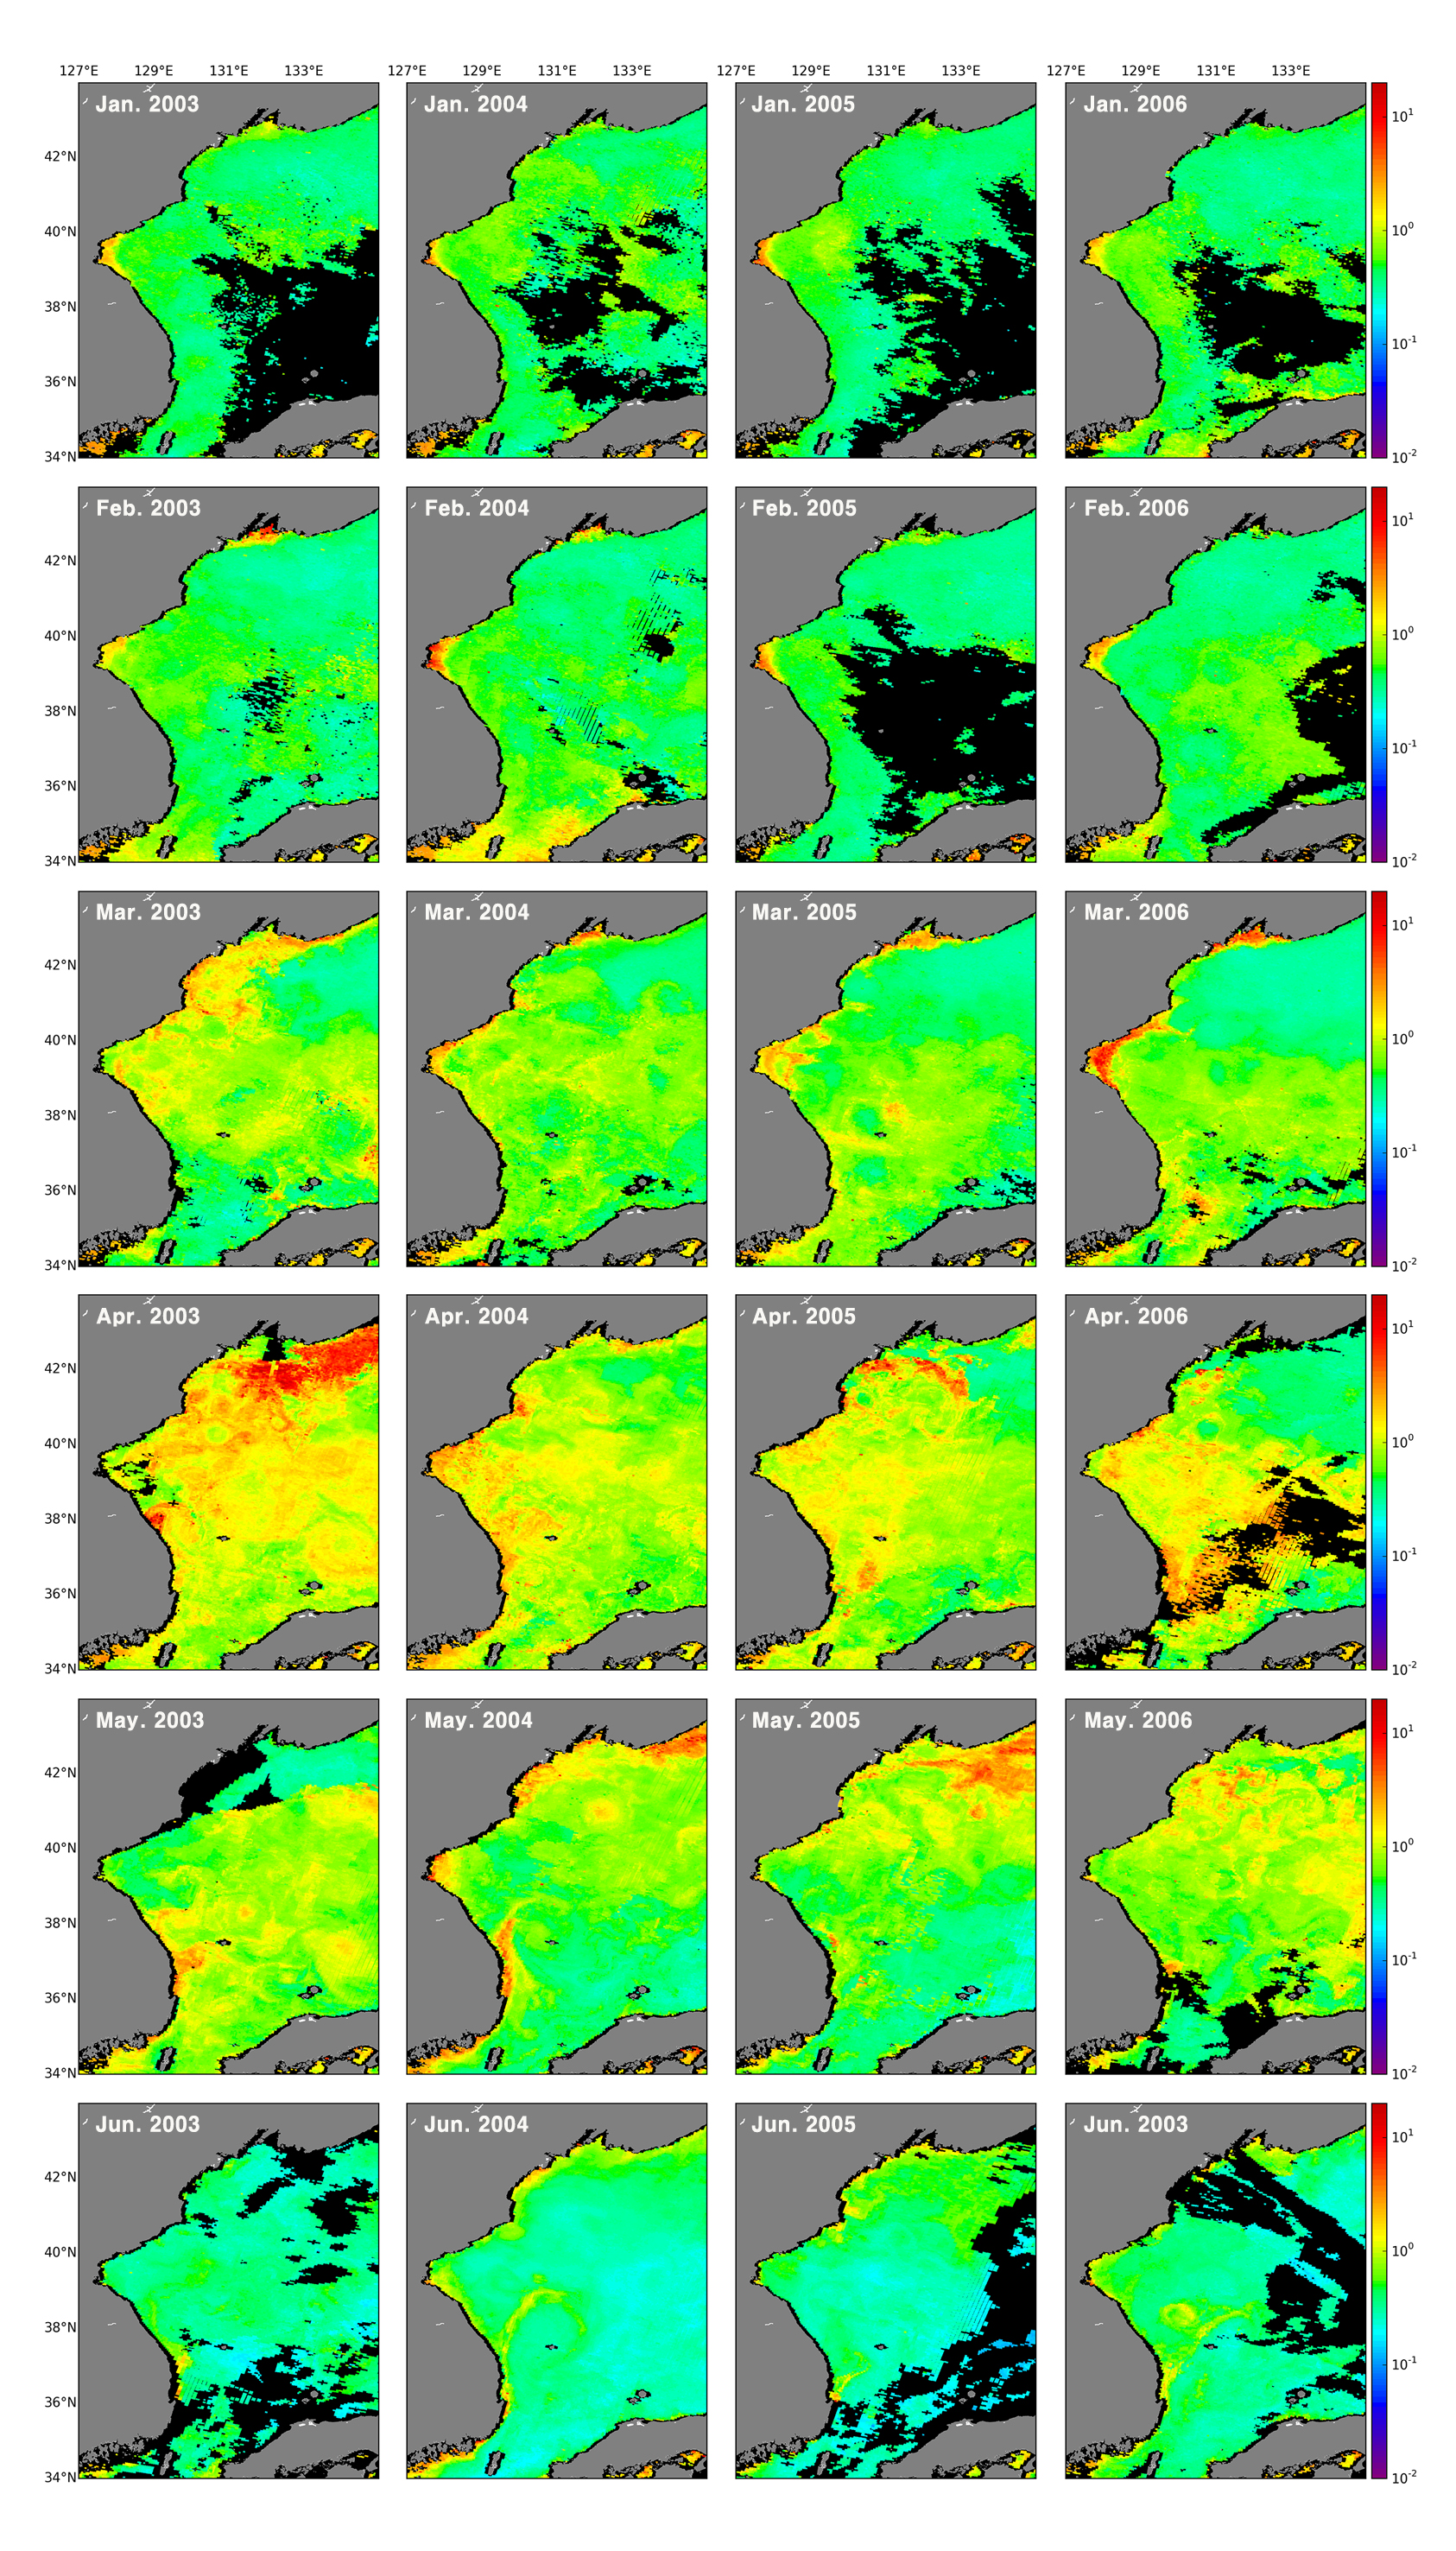
\includegraphics[width=0.8\linewidth]{../images/noname03}
	\caption{The monthly-mean chlorophyll-a distribution in the Korean East Sea, GAC. From 2003 to 2006, January to June. The unit of the color bar is $\rm mg/m^3$.}
	\label{fig:noname03}
\end{figure}

\begin{figure}
	\centering
	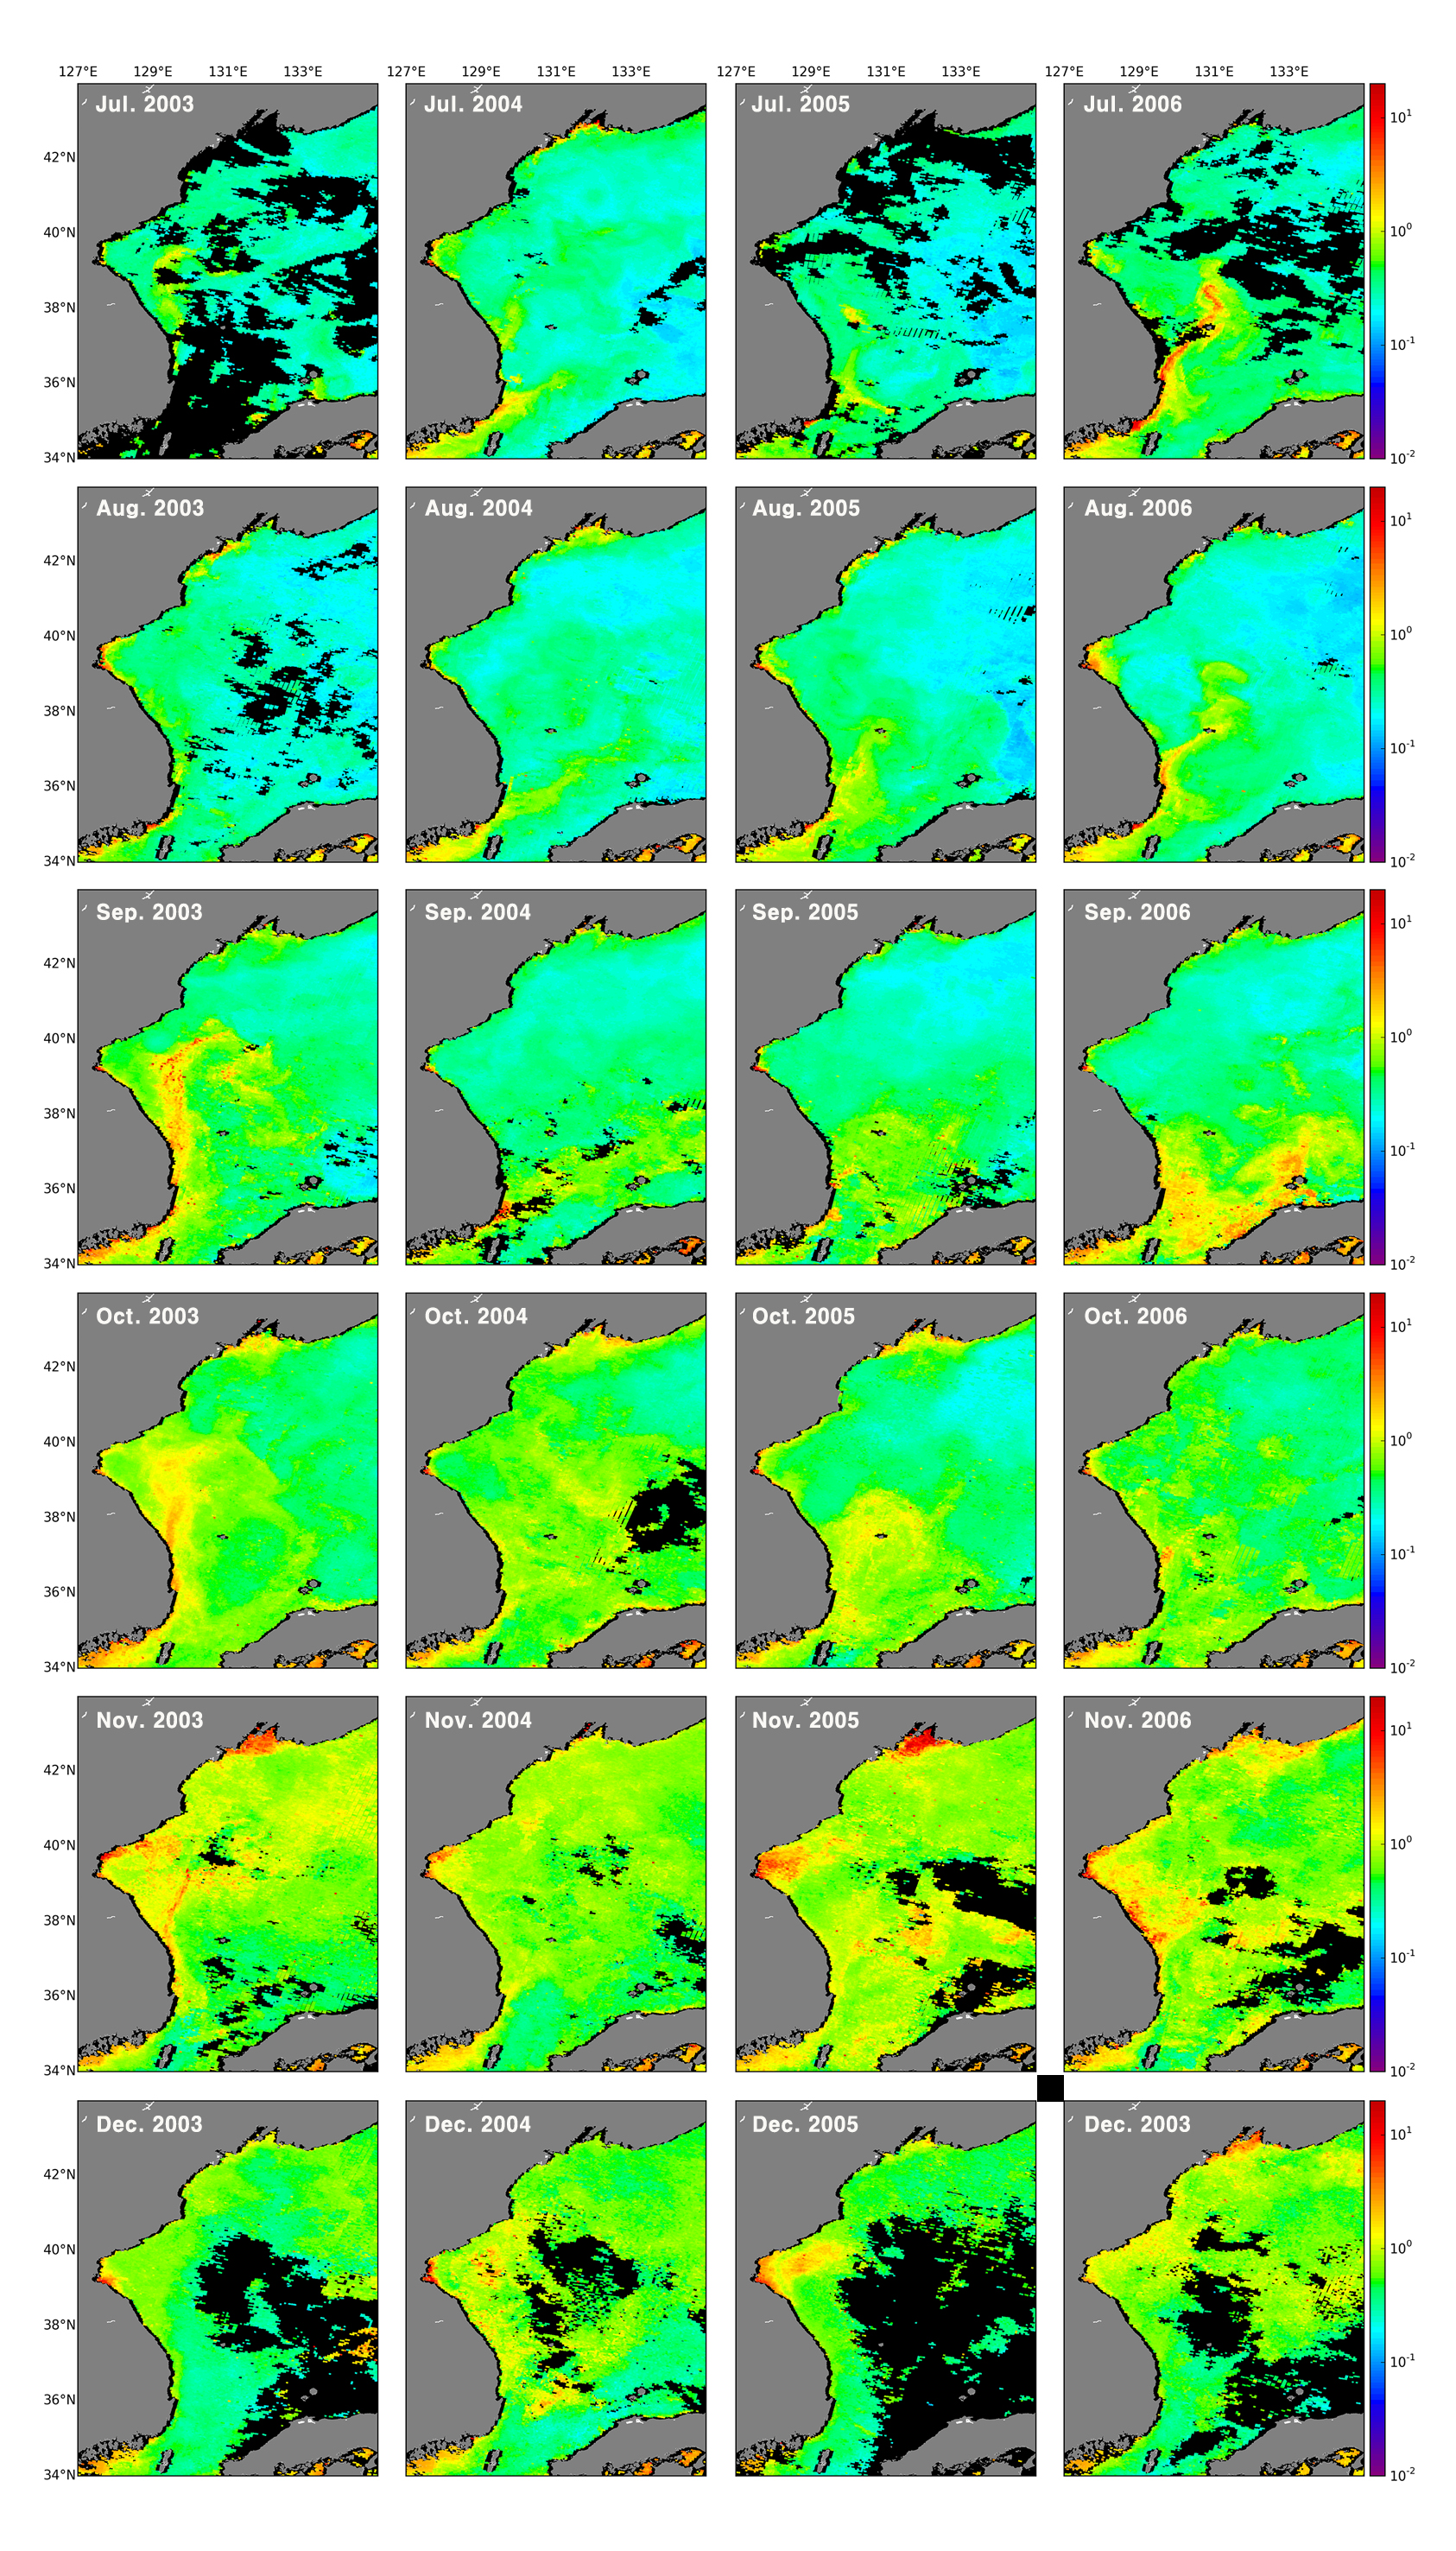
\includegraphics[width=0.8\linewidth]{../images/noname04}
	\caption{The monthly-mean chlorophyll-a distribution in the Korean East Sea, GAC. From 2003 to 2006, July to December. The unit of the color bar is $\rm mg/m^3$.}
	\label{fig:noname04}
\end{figure}
 
\subsection{The Effect of Spatial Resolution on the Data}
 
To find the effect of spatial resolution on the data, we compare the histograms of LAC data and the GAC data of April, 2003. We find that the histogram of GAC data shows more discontinuous shape compared to the LAC data in Figure.9. From the fact that a histogram of real data has continuous shape, it can be inferred that using LAC data is more accurate than using GAC data. The histogram of GAC data also shows more pixels with over 10 mg/m3 of chlorophyll-a concentration with sporadic distribution. These pixels are the speckles from previous researches (Chae, H. J., and Park, K., 2009; Hu, C., Carder, K. L., and Muller-Karger, F. E., 2001) also showing that LAC data is more appropriate for studying chlorophyll-a concentration.
  
  
  Figure 7 The monthly chlorophyll-a mean histogram in the Korean East Sea on April, 2003, (a) LAC (b) GAC.
  
  
   In Figure 10, part of the data with high chlorophyll-a concentration is enlarged to compare between LAC data and GAC data. LAC data has 6 pixels over 10 mg/m3, while GAC data has more than 100 pixels over 10 $\rm mg/m^3$. Such result occurs since one high-concentration value in GAC data affects a large area compared to LAC because of its low resolution.
  In Figure 11, part of the data with speckles is enlarged to compare between LAC data and GAC data. GAC data has a larger size of speckle because it has low resolution. In other words, it has more errors. Even if the speckles of the GAC data has been corrected, it will correct larger area compared to LAC causing a larger gap between the real value. In addition, even with the speckle correction applied using corrected LAC data will be more accurate.
  
  Figure 8. The monthly chlorophyll-a mean distribution in the Korean East Sea on April, 2003, (a) LAC (b) GAC. Enlarged an area with high concentrations of chlorophyll-a
  
  Figure 9. The monthly chlorophyll-a mean distribution in the Korean East Sea on April, 2003, (a) LAC (b) GAC. Enlarged an area with speckles
  
  
  
  